\documentclass[11pt,a4paper]{article}
\usepackage[top=3cm, bottom=2cm, left=2cm, right=2cm]{geometry}
\usepackage[utf8]{inputenc}
\usepackage{amsmath, amsfonts, amssymb}
\usepackage{siunitx}
\usepackage[brazil]{babel}
\usepackage{graphicx}
\usepackage[margin=10pt,font={small, it},labelfont=bf, textfont=it]{caption}
\usepackage[dvipsnames, svgnames]{xcolor}
\DeclareCaptionFont{MediumOrchid}{\color[svgnames]{MediumOrchid}}
\usepackage[pdftex]{hyperref}
\usepackage{natbib}
\bibliographystyle{plainnat}
\bibpunct{[}{]}{,}{s}{}{}
\usepackage{color}
\usepackage{footnote}
\usepackage{setspace}
\usepackage{booktabs}
\usepackage{multirow}
\usepackage{subfigure}
\usepackage{fancyhdr}
\usepackage{leading}
\usepackage{indentfirst}
\usepackage{wrapfig}
\usepackage{mdframed}
\usepackage{etoolbox}
\usepackage[version=4]{mhchem}
\usepackage{enumitem}
\usepackage{caption}
\usepackage{titlesec}
\usepackage{tcolorbox}
\usepackage{tikz}
\usepackage{LobsterTwo}
\usepackage[T1]{fontenc}
\usepackage{fontspec}
\usepackage{txfonts}
\AtBeginEnvironment{equation}{\fontsize{13}{16}\selectfont}


\titleformat{\section}{\LobsterTwo\LARGE\color{CarnationPink}}{\thesection.}{1em}{}
\titleformat{\subsection}{\LobsterTwo\LARGE\color{CarnationPink}}{\thesubsection}{1em}{}


\DeclareCaptionLabelFormat{figuras}{\textcolor{DarkTurquoise}{Figura \arabic{figure}}}
\captionsetup[figure]{labelformat=figuras}

\makeatletter
\renewcommand\tagform@[1]{\maketag@@@{\color{CarnationPink}(#1)}}
\makeatother

\renewcommand{\theequation}{Eq. \arabic{equation}}
\renewcommand{\thefigure}{Fig. \arabic{figure}}
\renewcommand{\thesection}{\textcolor{CarnationPink}{\arabic{section}}}

\setlist[itemize]{label=\textcolor{CarnationPink}{$\mathbf{\square}$}}

\setlist[enumerate]{label=\textcolor{CarnationPink}{\arabic*.}, align=left}


\newcounter{exemplo}

\NewDocumentEnvironment{exemplo}{ O{} }{%
\allowbreak
\setlength{\parindent}{0pt}
  \begin{mdframed}[
  leftline=true,
  topline=false,
  rightline=false,
  bottomline=false,
  linewidth=2pt,
  linecolor=CarnationPink,
  frametitlerule=false,
  frametitlefont=\LobsterTwo\large\color{CarnationPink},
  frametitle={\color{CarnationPink}\LobsterTwo\large #1},
  ]
}{%
  \end{mdframed}
}

\setlength{\fboxsep}{5pt}
\setlength{\fboxrule}{1.5pt}
\usepackage{float}
\renewcommand{\thefootnote}{\alph{footnote}}
\usepackage{url}
\hypersetup{
	colorlinks=true,
	linkcolor=DarkTurquoise,
	filecolor=DarkTurquoise,      
	urlcolor=DarkTurquoise,
	citecolor=DarkTurquoise,
	pdftitle={Especialista em Física da Radioterapia}
}
\pagestyle{fancy}
\fancyhf{}
\renewcommand{\headrulewidth}{0pt}
\rfoot{Página \thepage}

\title{\LobsterTwo\Huge{Dosimetria}}
\author{\LobsterTwo\Large{Dosimetria In-Vivo}\nocite{*}}
\date{\LobsterTwo{Dalila Mendonça}}
\begin{document}
	\maketitle

\section{Introdução}

	Com o crescente foco nos erros de radioterapia nos últimos anos, tem havido um interesse crescente na utilização da dosimetria in vivo como outra etapa no processo de controle de qualidade. O report da IAEA No 8 conclui:

  	\begin{exemplo}
		Até recentemente, a implementação clínica rotineira da dosimetria in vivo tem sido bastante limitada em muitos centros de radioterapia. No entanto, há um crescente interesse em estabelecer programas de dosimetria in vivo. Isso foi parcialmente motivado por uma série recente de acidentes de radioterapia em países industrializados que poderiam ter sido evitados se esses programas estivessem em vigor. Acredita-se que esta publicação forneça orientações adequadas para a preparação e implementação de programas de dosimetria in vivo para técnicas estacionárias em radioterapia. Uma vez estabelecida, a dosimetria in vivo se torna uma ferramenta de garantia da qualidade que pode ajudar a reduzir erros na administração da dose em pacientes de radioterapia. Em resumo, a dosimetria in vivo é uma ferramenta adequada para detectar erros na radioterapia, avaliar diferenças clinicamente relevantes entre as doses prescritas e administradas, documentar as doses recebidas por pacientes individualmente e cumprir requisitos estabelecidos por algumas regulamentações nacionais.
	\end{exemplo}
		
	A dosimetria in vivo tem dois objetivos principais:
	
	\begin{enumerate}
		\item Prevenir erros graves na administração da dose; e
		\item Comparar a dose superficial calculada com a dose superficial medida em cenários clínicos especiais.
	\end{enumerate}

	Exemplos de cenários especiais incluem match line para feixes de elétrons combinados, tratamentos de neuro-eixo e verificação da dose superficial em tratamentos de TBI e TSI. Sistemas de dosimetria in vivo, como TLD, OSLD, MOSFETs ou diodos, podem medir a dose pontual na superfície. Portanto, eles são predominantemente aplicados em tratamentos conformacionais 3D para fins de segurança (para inferir a dose em profundidade a partir da dose de superfície) e em tratamentos com IMRT ou elétrons para medições pontuais de dose superficial. O uso desses sistemas adiciona cerca de 5 a 10 minutos ao tempo de setup do paciente. As tolerâncias clínicas típicas são de 5\% para medições de qualidade e segurança de rotina. Para medições clínicas de dose superficial, geralmente não há uma tolerância especificamente declarada. O físico fornecerá ao médico um relatório de consultoria física por escrito, indicando a dose planejada, a dose medida e as estimativas da incerteza da medição da dose superficial a partir dos sistemas de comissionamento do feixe e de planejamento do tratamento. Com base nessas informações, o médico usará o julgamento clínico para determinar se a variação na dose medida é aceitável ou se modificações no tratamento são indicadas.

	Estão em andamento técnicos para criar sistemas de dosimetria in vivo mais automatizados, que também possam ser aplicados à tratamentos de IMRT e VMAT. Uma abordagem consiste em montar uma câmara de transmissão no cabeçote do acelerador logo abaixo do colimador multi-leaf (MLC) para medir a fluência. Esse sistema será capaz de identificar erros no padrão do MLC ou na dose administrada por fração, mas não poderá detectar erros no posicionamento do paciente (SSD, deslocamentos). Uma desvantagem adicional é que ele precisa ser desmontado para tratamentos que requerem compensadores externos (filtros, blocos) ou cones de elétrons. A segunda abordagem, já disseminada, é utilizar o painel eletrônico de imagens portal (EPID) para medir a fluência na saída do paciente. Embora esse método possa adicionar uma dose extra de radiação ao EPID, o que pode acelerar o envelhecimento do equipamento, ele pode detectar a maioria dos erros no posicionamento do paciente e na entrega do tratamento pelo aparelho. Um limite do uso do EPID está em campos muito grandes, que poderiam irradiar a parte eletrônica do EPID.

	Em resumo, a dosimetria in vivo é útil para medições de superfície em situações clínicas selecionadas e como recurso essencial de segurança para prevenir erros na prática clínica. À medida que mais sistemas automatizados de dosimetria in vivo se tornam disponíveis, o uso rotineiro desses sistemas para cada paciente e cada fração acrescentará outra camada de verificação de segurança e qualidade à entrega do tratamento.



\section{Dosimetria In-Vivo}

	A dosimetria in vivo é usada clinicamente para verificar durante o tratamento com que precisão a dose planejada é administrada ao paciente. Enquanto a Associação Americana de Físicos em Medicina (AAPM) TG-62, \textit{``Diode In-Vivo Dosimetry for Patients Receiving External Beam Radiation Therapy''}, vê a dosimetria in-vivo como complementar a um bom programa de controle de qualidade, desenvolvimentos mais recentes na compreensão dos modos de falha na entrega do tratamento e na radioterapia adaptativa levaram a uma maior atenção aos ganhos de segurança e qualidade que um programa de dosimetria in vivo pode gerar com um custo relativamente baixo por paciente.

	Os dosímetros in vivo podem ser divididos em três categorias:

	\begin{enumerate}
		\item Os \textcolor{DarkTurquoise}{\textbf{Dosímetros de superfície}} como por exemplo, dosímetros termoluminescentes (TLD), dosímetros luminescentes opticamente estimulados (OSLD), diodos, transistores de efeito de campo semicondutor de óxido de metal (MOSFET) são colocados na superfície do paciente para medir a dose de entrada no paciente em planos conformacionais 2D e 3D. Eles também podem ser utilizados de forma mais geral para verificar a dose da pele em áreas anatomicamente críticas (por exemplo, acima de cicatrizes ou na mama contralateral). Às vezes, esses dosímetros também tem sido utilizados para aplicações intracavitárias.
		
		\item Os \textcolor{DarkTurquoise}{\textbf{Dosímetros Implantáveis}} foram desenvolvidos para avaliar a dose in situ tanto para alvos de tratamento quanto para órgãos de risco. Devido ao seu tamanho, as suas propriedades radiográficas e seu processo invasivo para sua colocação, o uso de dosímetros implantáveis tem sido amplamente abandonado em favor da dosimetria por transmissão;
		
		\item Os \textcolor{DarkTurquoise}{\textbf{Dosímetros de Transmissão}} são detectores de fluência que podem ser colocados imediatamente abaixo dos colimadores terciários ou em uma região distal do feixe para detectar a fluência de saída do paciente. 
	\end{enumerate}

	A dosimetria in-vivo atende a quatro propósitos:

	\begin{enumerate}[label=\textcolor{CarnationPink}{\roman*.}]
		\item No controle de qualidade paciente-específico, a dosimetria in-vivo é utilizada para confirmar que a entrega do tratamento está dentro das tolerâncias especificadas na política de procedimento da instituição. A dosimetria in-vivo pode ser utilizada com um diodo, um dosímetro implantável ou através de um sistema de dosimetria por transmissão como o EPID. Os resultados destas medidas devem ser revisados regularmente, geralmente durante as verificações semanais, a menos que os resultados sejam processados por meio de uma análise de um software que gera alertas para o usuário. Para dosímetros com leituras instantâneas, como os diodos e o MOSFET, um intervalo esperado deve ser fornecido para os operadores para que eles percebam imediatamente uma dose inesperada.
		
		\item Além do QA paciente-específico, os diodos também podem ser utilizados como QA de entrega (DQA) para tratamentos conformacionais 2D e 3D. Originalmente, eles pretendiam encontrar erros grosseiros, como filtro ausente ou incorreto, erros de setup envolvendo distância da fonte à superfície (SSD) ou erros na mesa de tratamento e erros nos parâmetros de tratamento que eram inseridos manualmente. Com a implementação de intertravamentos, tabelas de tolerância de mesa e sistemas R\&V automatizados usando algoritmos de soma de verificação para verificar a transferência de dados, conforme recomendado no ``International Electrotechnical Commission (IEC) report Medical Electrical Equipment—Requirements for the Safety of Radiotherapy Treatment Planning Systems'', a função DQA de diodos tornou-se menos crítica para a segurança na última década.
		
		\item Para DQA em campos de radioterapia de intensidade modulada (IMRT) ou terapia de arco modulado volumétrico (VMAT), a dosimetria in-vivo é realizada usando dosimetria de transmissão com dispositivos posicionados abaixo do colimador terciário. Este controle pode ser entendido como uma continuação do DQA pré-tratamento, que é habitual nas técnicas de IMRT. Como tal, seu uso pode se tornar mais frequente à medida que o planejamento adaptativo e os cálculos rápidos de dose se tornam cada vez frequentes na rotina clínica.
		
		\item A dosimetria in vivo com dosímetros superficiais é realizada onde as incertezas nos cálculos do TPS e/ou no setup causam grandes incertezas na dose superficial que é relevante para o resultado do tratamento.
	\end{enumerate}

	O documento \textit{``European Society for Radiotherapy and Oncology (ESTRO) booklet on methods for in-vivo dosimetry''} fornece uma descrição completa e referências para os dosímetros de superfície e o documento \textit{``l Atomic Energy Agency (IAEA) Human Health Report No. 8, Development of Procedures for In Vivo Dosimetry in Radiotherapy''} também fornece uma descrição detalhada da tecnologia do detector e também descreve o processo de implementação da dosimetria in-vivo e relata os resultados de um programa piloto em seis países e quatro continentes.


\section{Processo Clínico}

\subsection{Implementação do Sistema}

	A IAEA recomenda um físico médico qualificado (QMP) para ser o principal responsável pela criação e supervisão de um programa de dosimetria in-vivo. Para estabelecer um processo clínico de qualidade, é necessária a contribuição dos médicos quanto ao estabelecimento de níveis de ação clínicos adequados. Além disso, a equipe dos técnicos deve estar envolvida na avaliação do sistema de dosimetria in-vivo para facilidade e praticidade de uso na prática  diária. A IAEA fornece um exemplo de fluxograma para a configuração do processo, que pode ser adaptado para um procedimento clínico.

	O processo de comissionamento de qualquer sistema de dosimetria in-vivo deve caracterizar o desempenho do detector para a faixa de parâmetros necessários para o uso clínico. A 
	calibração e a medida dos fatores de correção são normalmente realizadas em água sólida. Para o processo de verificação, as medições de feixes padrão incidentes em um phantom  antropomórfico devem ser seguidas pela verificação em planos de pacientes usados clinicamente em um phantom antropomórfico. A \ref{fig:medidasDosimetrosInVivo} fornece um breve resumo dos testes de comissionamento.

	\begin{figure}[h]
		\centering
		\fcolorbox{DarkTurquoise}{white}{%
			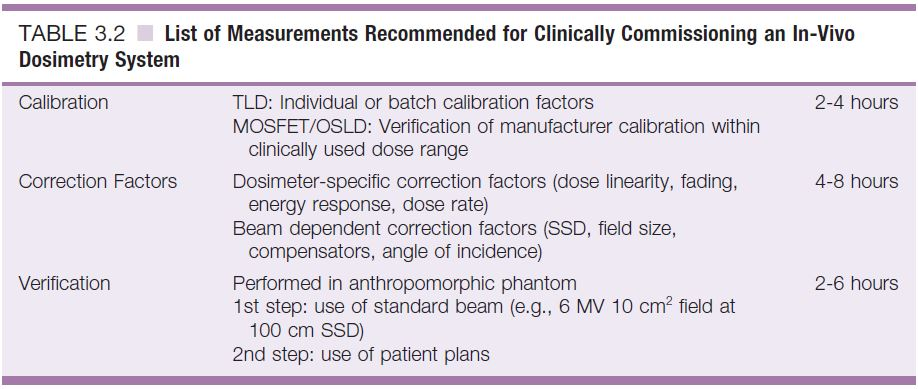
\includegraphics[width=0.9\textwidth]{Imagens/medidasDosimetrosInVivo.JPG}
		}%
		\caption{Testes de comissionamento para dosimetria in-vivo}
		\label{fig:medidasDosimetrosInVivo}
	\end{figure}

\subsection{Níveis de Ação}

	Os níveis de tolerância e os níveis de ação precisam ser definidos de modo que sejam clinicamente e tecnicamente significativos. A Comissão Internacional de Unidades e Medidas de Radiação (ICRU) definiu 5\% de desvio da dose planejada como um limite de ação aceitável, que foi enfatizado novamente pelo TG-40, \textit{``Comprehensive QA for Radiation Oncology''}. Com isso em mente, a IAEA estabeleceu 5\% como limite de ação para seu estudo piloto de dosimetria in vivo. É uma prática clínica estabelecida, definir um nível de tolerância abaixo do nível de ação, o que serve como um sinal no processo de revisão do QA de que existem parâmetros críticos que estão tendendo para o limite de ação. Esse nível de tolerância é diferente para cada clínica com base no equipamento disponível e na experiência do usuário. O método padrão da indústria para definir um nível de tolerância apropriado específico do local é o controle estatístico do processo.

\section{Dosímetros de Superfície}

\subsection{Finalidade e Calibração}

	Os dosímetros de superfície são usados para medir a dose de entrada e saída do paciente, embora o último seja raramente feito devido à dificuldade em colocar um detector de forma confiável e confortável embaixo do paciente.

	Os dosímetros de superfície para DQA in vivo podem ser classificados em duas finalidades:

	\begin{enumerate}[label=\textcolor{CarnationPink}{\arabic*${}^\circ $}]
		\item Medidas da dose na pele;
		\item Medidas da dose na superfície para inferir a dose na profundidade;
	\end{enumerate}

	Historicamente, o uso predominante da dosimetria in vivo eram em medidas da dose superficial no paciente tratamentos 2D e 3D para inferir a dose na profundidade. Com sistemas modernos de registro e verificação (Record \& Verify - R\&V), o advento dos colimadores multilâminas (MLCs), setups guiados por imagem, substituição de filtros físicos por filtros universais ou dinâmicos, juntamente com melhores sistemas de segurança analógicos e eletrônicos, o uso rotineiro de dosímetros de superfície para verificação de dose na profundidade tornou-se menos comum. No entanto, como aponta o Relatório de Saúde Humana nº 8 da IAEA, o sistema de R\&V controla apenas os parâmetros inseridos no software; os erros originados no planejamento do tratamento ou no setup do paciente não são detectados. Portanto, a IAEA recomenda a implementação da dosimetria in-vivo para todos os pacientes.

	A medida da dose na superfície para inferir a dose em profundidade é um padrão clínico aceito para procedimentos especiais e em casos como a verificação do posicionamento correto dos compensadores de chumbo e o cálculo da dose na distância estendida em um tratamento de \textit{`Total Body Irradiation (TBI)''}. Os dosímetros in-vivo usados para inferir a dose na profundidade são calibrados em um simulador usando um segundo detector em uma profundidade predefinida, geralmente igual a $d_{max}$. A \ref{fig:setupCalibracaoDosimInVivo} mostra a configuração de calibração para um dosímetro in vivo usado para inferir a dose em profundidade. As leituras in-vivo do dosímetro são calibradas de forma cruzada com a dose medida por um segundo dosímetro colocado em profundidade no phantom. Para tornar a leitura do detector mais robusta na região de buildup onde existe um alto gradiente de dose, pode ser utilizado uma capa de buildup ou um pequeno bolus. Alguns diodos são desenvolvidos para fornecer um buildup inerente afim de atingir esse objetivo.

	\begin{figure}[h]
		\centering
		\fcolorbox{DarkTurquoise}{white}{%
			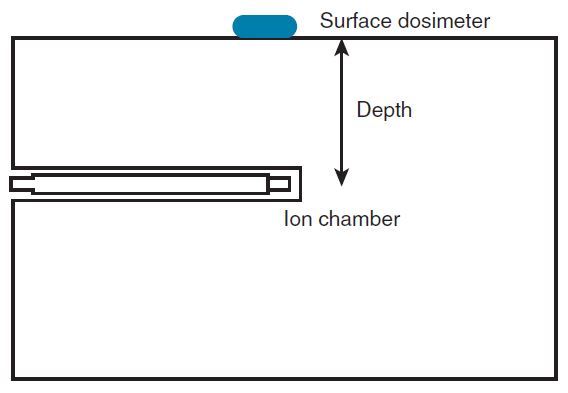
\includegraphics[width=0.8\textwidth]{Imagens/setupCalibracaoDosimInVivo.JPG}
		}%
		\caption{Setup para calibração dos dosímetros superficiais para medir a dose na profundidade.}
		\label{fig:setupCalibracaoDosimInVivo}
	\end{figure}

	O uso de métodos para verificar a dose planejada na pele é motivado pelas grandes incertezas ao medir os dados do feixe na região de buildup durante o comissionamento e o desafio de modelar a região de buildup com precisão em sistemas de planejamento. A medida da dose na pele é utilizada para verificar a dose nas cicatrizes cirúrgicas que precisam ser irradiadas para evitar a recorrência da doença disseminada. A dose na pele em tratamentos superficiais, como \textit{``Total Skin Irradiation (TSI)''} para micose fungóide, melanomas e tumores que invadem a pele, são outras aplicações da medida da dose superficial. De acordo com ICRU-35, o ponto de medida na pele é definido como 0.5 mm abaixo da superfície. Para dosímetros in-vivo com superfície muito fina, deve ser usado um buildup de 0.5 mm, como cera odontológica, por exemplo. O \textit{``Human Health Report No. 8''} da IAEA recomenda limitar a atenuação do feixe causada pelo dosímetro para um valor $<$ 5\% para minimizar a perturbação da dose no alvo.

	Para cada tipo de detector, os fatores de correção devem ser estabelecidos com base nas propriedades físicas do detector. Todos os detectores de radiação mostram uma não linearidade na resposta com respeito a dose nos extremos baixo e alto da faixa de atuação de do detector. Portanto, uma curva de resposta em função da dose deve ser estabelecida como parte do comissionamento do dosímetro in-vivo. Da mesma forma, as características da resposta do detector em função da energia do feixe devem ser estabelecidas para a faixa de energias de feixe nas quais o dosímetro será utilizado. O comissionamento de um sistema de dosimetria in-vivo deve incorporar um estudo cuidadoso da resposta do dosímetro em função de todas as taxas de dose intrínsecas disponíveis, bem como as taxas de dose encontradas ao longo da faixa de SSDs utilizadas na rotina. Este último é especialmente importante para a dosimetria in-vivo de tratamentos de TBI em SSDs estendidas. Alguns dosímetros, como o TLD e os filmes radiocrômicos, apresentam uma mudança na resposta para a leitura em função do tempo. A menos que um intervalo de tempo padronizado entre a medida e a leitura possa ser estabelecido, essa resposta à dose dependente do tempo também precisa ser caracterizada.

	Dois fatores de correção dependem do feixe:

	\begin{enumerate}
		\item A alteração do espalhamento e da contaminação com elétrons que atingem o dosímetro de superfície à medida que o tamanho do feixe ou a distância foco-superfície (SSD) mudam. A IAEA recomenda avaliar a dependência do tamanho do campo e da SSD ao longo da faixa de energias de feixes utilizados clinicamente; se os fatores de correção excederem 1\%, eles devem ser aplicados nas medidas clínicas.
		
		\item A correção em função do ângulo de incidência, que pode ser necessária ao medir feixes com ângulos de incidência fortemente inclinados (por exemplo, em tratamentos de mama ou parede torácica). Assim como no primeiro fator, a IAEA recomenda aplicar este fator apenas se as medidas mostrarem que é necessária uma correção superior a 1\%.
	\end{enumerate}
	
	A \ref{fig:dosimetrosInVivo} resume os dosímetros in-vivo atualmente utilizados e suas principais características.

	\begin{figure}[h]
		\centering
		\fcolorbox{DarkTurquoise}{white}{%
			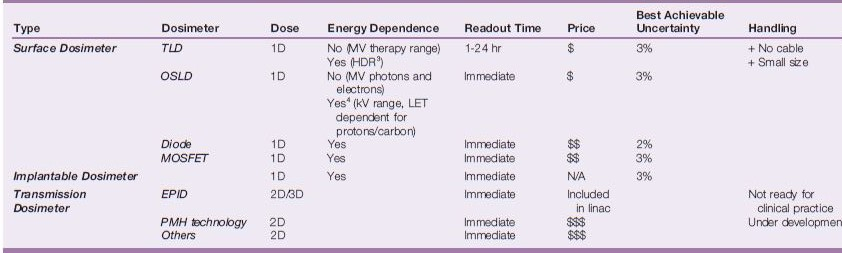
\includegraphics[width=0.8\textwidth]{Imagens/dosimetrosInVivo.JPG}
		}%
		\caption{Dosímetros In-vivo.}
		\label{fig:dosimetrosInVivo}
	\end{figure}



\subsection{Dosímetros Termoluminescentes}

	Atualmente, existem dois tipos de materiais de TLD amplamente utilizados na prática clínica:
	
	\begin{enumerate}[label=\textcolor{CarnationPink}{\arabic*${}^\circ $}]
		\item \textcolor{DarkTurquoise}{\textbf{(LiF:Mg, Ti)}}, que tem resposta linear com a dose até 1 Gy e resposta supra-linear acima de 1 Gy; e
		\item \textcolor{DarkTurquoise}{\textbf{(LiF:Mg, Cu, P)}}, que tem resposta linear com a dose até 10 Gy e resposta sublinear acima de 10 Gy.
	\end{enumerate}
	
	Durante o processo de comissionamento, a curva de linearidade de dose deve ser verificada dentro da faixa de dose clinicamente esperada. O (LiF:Mg, Ti) é menos sensível aos processamentos térmicos do que o (LiF:Mg, Cu, P), o que o tornou a escolha preferida de material TLD até que se tornassem disponíveis fornos programáveis para que fosse possível manter os padrões de recozimento (``annealing'') consistentes. Os TLDs podem ser fabricados em vários formatos e tamanhos; pós, cubos, chips e bastões são os mais comumente disponíveis. Dependendo da forma, pode haver uma dependência angular caso a superfície do TLD não tenha sido cuidadosamente posicionada em relação ao ângulo de incidência do feixe.  Na prática clínica, a melhor opção é medir a resposta em função da dose para todas as energias de feixe disponíveis afim de determinar se pode ser necessário um fator de correção para a energia pois, existe uma literatura extensa e às vezes contraditória sobre a dependência energética dos TLDs\dots



	\begin{tcolorbox}[width=\textwidth, colback={white}, colbacktitle={DarkTurquoise!50!white}, title={$\bigstar$ \LobsterTwo{Nota:} $\bigstar $}, coltitle={CarnationPink}, colframe={DarkTurquoise}, fonttitle=\rmfamily\bfseries\Large]
		$\quad$ O termo ``annealing'' refere-se ao processo de recozimento térmico de um material, geralmente realizado em temperaturas elevadas, seguido por um resfriamento controlado. Esse processo é utilizado para modificar as propriedades físicas do material, como sua estrutura cristalina e a distribuição de defeitos internos, a fim de melhorar suas características e desempenho. 
	\end{tcolorbox}

	A principal desvantagem dos TLDs é o decaimento das armadilhas de elétrons de baixa energia à temperatura ambiente (fading, ``desvanecimento''). Três estratégias principais podem ser empregadas clinicamente para gerenciar o efeito do desvanecimento da precisão da medida da dose:

	\begin{enumerate}[label=\textcolor{CarnationPink}{\arabic*${}^\circ $}]
		\item Lendo o TLD dentro de uma janela temporal bem definida em um intervalo de tempo específico após a medida.
		\item Pré-recozimento antes da leitura (ou seja, aquecimento do TLD usando um padrão de baixa temperatura específico para forçar o decaimento das armadilhas de elétrons de baixa energia).
		\item Lendo os TLDs pelo menos 24 horas após a medida pois este é o tempo em que a maioria dos elétrons de baixa energia já decaíram.
	\end{enumerate}

	A leitura é realizada submetendo o TLD a um padrão de aquecimento bem definido e medindo a luminescência das curvas luminosas resultantes. As curvas luminosas de baixa energia são geralmente descartadas nas leitura por pré-recozimento, no desvanecimento à temperatura ambiente ou subtraindo eletronicamente da saída de luz na faixa de baixa temperatura da curva de leitura. Para manter uma relação constante entre luminescência e dose lida, deve-se tomar muito cuidado para manter a superfície do TLD limpa e sem danos. Os TLDs devem ser manuseados apenas com ferramentas e/ou luvas limpas para evitar a contaminação da superfície por óleos e células da pele. Os TLDs arranhados ou lascados também devem ser eliminados do uso clínico.

	Dois métodos de calibração são utilizados na rotina clínica:

	\begin{enumerate}
		\item Cada TLD é calibrado individualmente. Os fatores de calibração são armazenados em um banco de dados e aplicados a cada leitura. A vantagem é a precisão muito alta da medida da dose; a desvantagem é o fardo administrativo adicional de rastrear individualmente cada TLD e o risco de trocar acidentalmente de TLDs ao manipulá-los.
		
		\item Os TLDs são calibrados e classificados em lotes. Para este método, um lote de TLDs é irradiado e dividido em lotes menores com base em seu respectivo fator de calibração. A vantagem é o manuseio e rastreamento mais fácil dos TLDs agrupados; a desvantagem é uma dispersão ligeiramente maior na incerteza na medida da dose, dependendo do número de TLDs no lote original e a dispersão da resposta em função da dose nos sub-lotes.
	\end{enumerate}

\subsection{Dosímetros Luminescentes Opticamente Estimulados}

	Os dosímetros de luminescência opticamente estimulada (OSLDs) são feitos de óxido de alumínio dopado com carbono (\ce{Al2O3}:\ce{C}) e foram usados primeiramente na dosimetria pessoal antes de serem aplicados no ambiente clínico. Eles são muito semelhantes aos TLDs, pois são dosímetros passivos de tamanho pequeno que podem ser aplicados à faixa de doses e energias de feixe encontradas em imagens e tratamentos com raios-x. Ao contrário dos TLDs, a luminescência para leitura de OSLDs não requer calor, apenas estimulação óptica. Definindo cuidadosamente os parâmetros de leitura, a depleção do sinal do OSLD pode ser reduzida ao mínimo, permitindo assim leituras repetidas quase não destrutivas da dose medida. A precisão e a consistência das leituras repetidas de acordo com as especificações do fabricante devem ser verificadas como parte do processo de comissionamento do OSLD. Estudos sobre a determinação dos limites superiores de dose cumulativa ainda estão em andamento e alguns estudos indicam que OSLDs não devem ser usados para irradiações repetidas sem primeiro foto-branquear o OSLD sob luz intensa.

\subsection{Diodos}

	O TG-62 e o Capítulo 28 da 2009 AAPM Summer School fornecem um resumo dos diodos de silício usados como detectores de radiação in vivo. Os detectores de diodo são pequenos, têm alta sensibilidade à radiação e são fisicamente robustos, tornando-os muito adequados para uso frequente na prática clínica.

	A mudança na recombinação indireta é o efeito dominante que altera a resposta do diodo, ocorrendo sob três condições:

	\begin{enumerate}[label=\textcolor{CarnationPink}{\arabic*${}^\circ $}]
		\item Dano físico ou por radiação do material do diodo;
		\item Aumento da taxa de dose instantânea;
		\item Mudanças na temperatura.
	\end{enumerate}

	A primeira é a razão pela qual os diodos se deterioram com o uso, levando a uma vida útil finita como ``detectores úteis'', dependendo da dose cumulativa e da energia da radiação. A segunda causa efeitos de taxa de dose, que podem ser especialmente pronunciados para linacs com alta taxa de dose instantânea. Os efeitos da taxa de dose também podem ser observados em medidas em várias SSDs ou com atenuadores de feixe. A recombinação indireta é fortemente dependente do material do detector. Para diminuir as mudanças na resposta à radiação ao longo da vida útil do diodo, os fabricantes geralmente introduzem, intencionalmente, defeitos na estrutura do cristal através de dopagem com metais (por exemplo, platina) e/ou através da pré-irradiação dos diodos. Isto resulta em uma redução na resposta do diodo que é considerada aceitável pois deste modo é possível obter maior estabilidade na resposta.

	O próprio material do diodo é fabricado em um disco fino chamado \textit{``die''} (matriz/chip). A própria matriz é embalada, geralmente com material adicional para buildup com diferentes espessuras, dependendo da energia do feixe que será utilizada. Se os diodos forem utilizados para dosimetria in-vivo em tratamentos de TBI, os efeitos da maior componente de baixa energia do feixe na SSD estendida devem ser avaliadas. O próprio fator da forma do diodo causa uma dependência direcional na sua resposta, que pode ser amplificada dependendo da construção do buildup. O material da embalagem também pode influenciar a dependência energética do diodo, como mostra a \ref{fig:testesDiodo}.

	\begin{figure}[h]
		\centering
		\fcolorbox{DarkTurquoise}{white}{%
			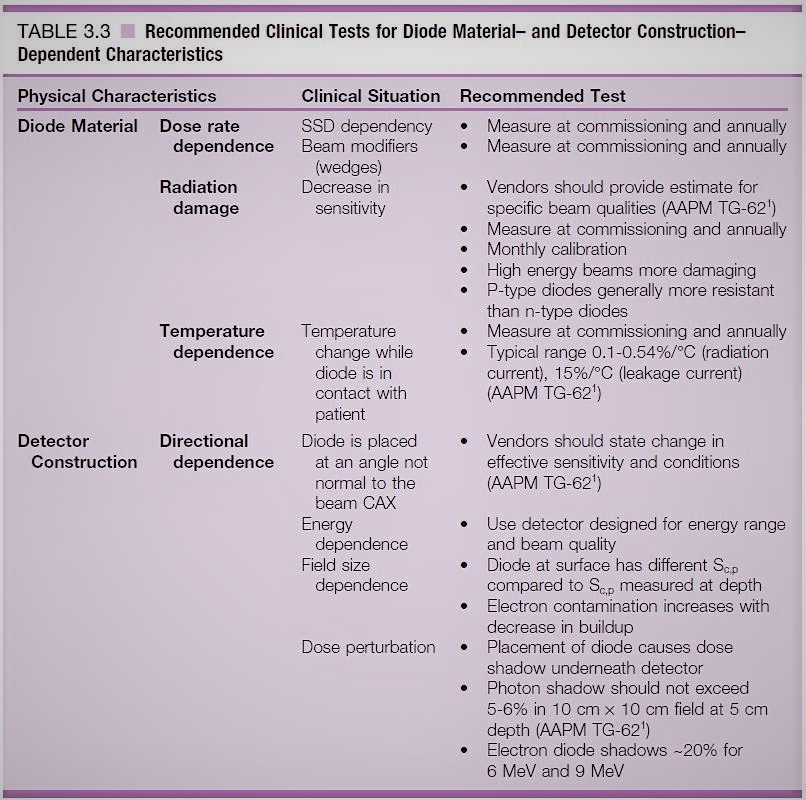
\includegraphics[width=0.8\textwidth]{Imagens/testesDiodo.JPG}
		}%
		\caption{Testes clínicos recomendados para características dependentes do material do diodo e da construção do detector}
		\label{fig:testesDiodo}
	\end{figure}

\subsection{MOSFETs}

	Os detectores transistores de efeito de campo em semicondutores de óxido de metal (MOSFETs) são transistores que podem funcionar no modo passivo (sem tensão aplicada durante a medição) ou ativo (polarizado). Ambos os modos têm sido usados para dosimetria in vivo.
	
	As vantagens dos MOSFETs são seu tamanho pequeno e sua capacidade de leitura em tempo real semelhante aos diodos. A sua desvantagem é que estes detectores saturam com a dose, exigindo um rastreamento preciso da dose cumulativa para sistemas MOSFET. Devido a essa saturação de dose, os detectores MOSFET geralmente são pré-calibrados pelo fabricante. Portanto, as medidas de comissionamento geralmente são cuidadosamente projetadas para limitar o acúmulo de dose no sistema clínico. Os fabricantes também fornecem limites superiores de dose cumulativa acima dos quais a linearidade da resposta à dose não é garantida. A maioria dos sistemas MOSFET também exibe dependência com a temperatura, embora os projetos contendo  circuitos duplo de detector de polarização dupla tenham reduzido o efeito da temperatura. A dependência energética e a dependência angular dos MOSFETs se comportam de maneira muito semelhante aos diodos.

\subsection{Detectores de Diamante}

	Os detectores de diamante podem ser fabricados em tamanhos pequenos e quase não apresentam dependência energética na faixa de energia utilizada na rotina clínica. Devido à baixa disponibilidade e alto custo, seu uso até agora foi restrito a centros acadêmicos selecionados, e existem poucas publicações relatando possíveis aplicações para dosimetria in vivo (até 2016).

\section{Dosímetros Implantáveis}

	Os dosímetros in vivo abordados fornecem apenas dados pontuais na superfície de entrada ou  na saída do paciente. A partir deles, a precisão da dose alvo é inferida. Os dosímetros implantáveis são projetados para medir diretamente a dose no alvo. Para alvos ao redor de cavidades (por exemplo, câncer de esôfago), podem ser usados dosímetros de superfície em embalagens à prova d'água. Uma técnica semelhante - implantar e posteriormente remover os dosímetros por meio de cirurgia - tem sido usada em pesquisas com animais, mas essa abordagem é claramente proibitiva na prática clínica em humanos. Os sistemas que estavam no mercado foram descontinuados e, atualmente, nenhum sistema de dosimetria implantável está disponível comercialmente.

\section{Dosimetria por Transmissão}

	Os dosímetros de transmissão foram desenvolvidos para fornecer informações dosimétricas 2D ou informações dosimétricas 3D com algoritmos de reconstrução de dose. Eles podem ser usados para tratamentos conformacionais 3D, IMRT e VMAT. Os dosímetros de transmissão se enquadram em duas categorias gerais:
	
	\begin{enumerate}
		\item Aqueles montados no gantry abaixo do MLC, que medem a dose de entrada no paciente; e
		\item Aqueles que medem a dose de saída do paciente.
	\end{enumerate}
	(1)  e (2) 

\subsection{Fluência de Entrada no Paciente}

	Os dosímetros de transmissão para avaliar a dose de entrada no paciente são posicionados utilizando os acessórios para fixar os cones de elétrons ou bandejas. Como eles devem ser removidos caso seja necessário utilizar outros acessórios acessórios, eles devem ser construídos dentro de um limite de peso razoável para o técnico levantar e também serem bastante robustos quanto ao manuseio para evitar danos. Os dosímetros de transmissão de dose de entrada são usados para verificar a dose antes de incidir no paciente (ou seja, seu objetivo é o controle de qualidade da máquina).

\subsection{Dose de Saída do Paciente}

	Os EPIDs são usados como dosímetros de transmissão para avaliar a saída de dose do paciente, além de sua finalidade principal de aquisição de imagens. Os componentes eletrônicos do EPID são sensíveis à radiação do feixe primário direto, o que limita o tamanho de campo máximo permitido para a dosimetria com EPID sendo a área ativa do detector de silício amorfo. A vantagem da dosimetria in vivo da dose de saída em comparação com a dosimetria in vivo da dose de entrada é a informação adicional sobre a perda de fluência no paciente. No entanto, isso também torna mais complicado distinguir erros de entrega da máquina e incertezas introduzidas por erros de setup do paciente e movimento respiratório.


\bibliography{ref.bib}
\end{document}